\chapter{Metodologia}

O processo metodológico empregado neste trabalho descreve as fases e estratégias adotadas. Ele foi concebido com a finalidade de alcançar os resultados propostos e responder às questões da pesquisa formuladas.

\section{Estratégia de Pesquisa}

A estratégia de pesquisa escolhida para este trabalho foi baseada em uma mescla de pesquisa exploratória, revisão bibliográfica e desenvolvimento prático. A pesquisa exploratória foi executada para obter um entendimento mais profundo do tema, identificar os conceitos-chave e tendências, e averiguar as soluções existentes. A revisão bibliográfica foi executada para examinar e analisar as principais publicações, artigos acadêmicos e normas associadas ao WoTPy e ao W3C-WoT. Isso forneceu fundamentação teórica para o trabalho e identificou brechas ou possibilidades de aprimoramento. O desenvolvimento prático incluiu a implementação e teste do WoTPy e a elaboração de exemplos de uso e documentação extensa.

\section{Coleta de Informações}

A coleta de informações foi feita por meio de várias fontes, como artigos acadêmicos, publicações, documentação oficial do W3C-WoT e WoTPy, e experimentos práticos. A revisão literária foi realizada para reunir dados relevantes sobre o W3C-WoT, as tecnologias envolvidas, os padrões e as práticas recomendadas. A documentação oficial do W3C-WoT \citeonline{Architecture} e do WoTPy \citeonline{wotpy} foi analisada para entender as especificações, APIs e diretrizes sugeridas.

\section{Elaboração do WoTPy}

A elaboração do WoTPy foi conduzida com base nas especificações e diretrizes do W3C-WoT. Primeiramente, foi feita uma análise minuciosa das especificações do W3C-WoT para compreender os conceitos essenciais e requisitos. Em seguida, foram escolhidas as bibliotecas e ferramentas apropriadas como dependências do WoTPy. Foram solucionados problemas de instalação e configuração para assegurar a facilidade de implementação em diferentes ambientes e sistemas operacionais. A elaboração do WoTPy foi feita utilizando a linguagem de programação Python e seguindo as melhores práticas de desenvolvimento de \textit{software}.

\section{Verificação e Testes}

A verificação do WoTPy foi feita por meio de um conjunto de testes disponíveis no repositório wot-py \citeonline{gitwotpy:2022}.

\section{Elaboração do Exemplo de Uso e Documentação}

Para ajudar os desenvolvedores e usuários na implementação do WoTPy em seus projetos IoT, foi elaborado um exemplo de uso prático e documentação. O exemplo de uso abrange cenários comuns de aplicação do WoTPy, demonstrando como utilizar suas funcionalidades e integrar dispositivos IoT. A documentação oferece informações sobre a instalação e configuração, para a utilização do WoTPy.

\section{Programação}

O trabalho foi realizado em fases sequenciais, com uma programação estabelecida para guiar o progresso e a organização das atividades, conforme demonstrado na figura \ref{fig:cronograma}.

Cada fase foi planejada para ser finalizada dentro de um período de tempo específico, possibilitando o avanço constante do trabalho e o cumprimento dos prazos fixados.

\begin{figure}
    \caption{Cronograma}
    \label{fig:cronograma}
    % trim={<left> <lower> <right> <upper>}
    % fonte da figura: https://www.overleaf.com/8438582545qhnjttttmmtn
    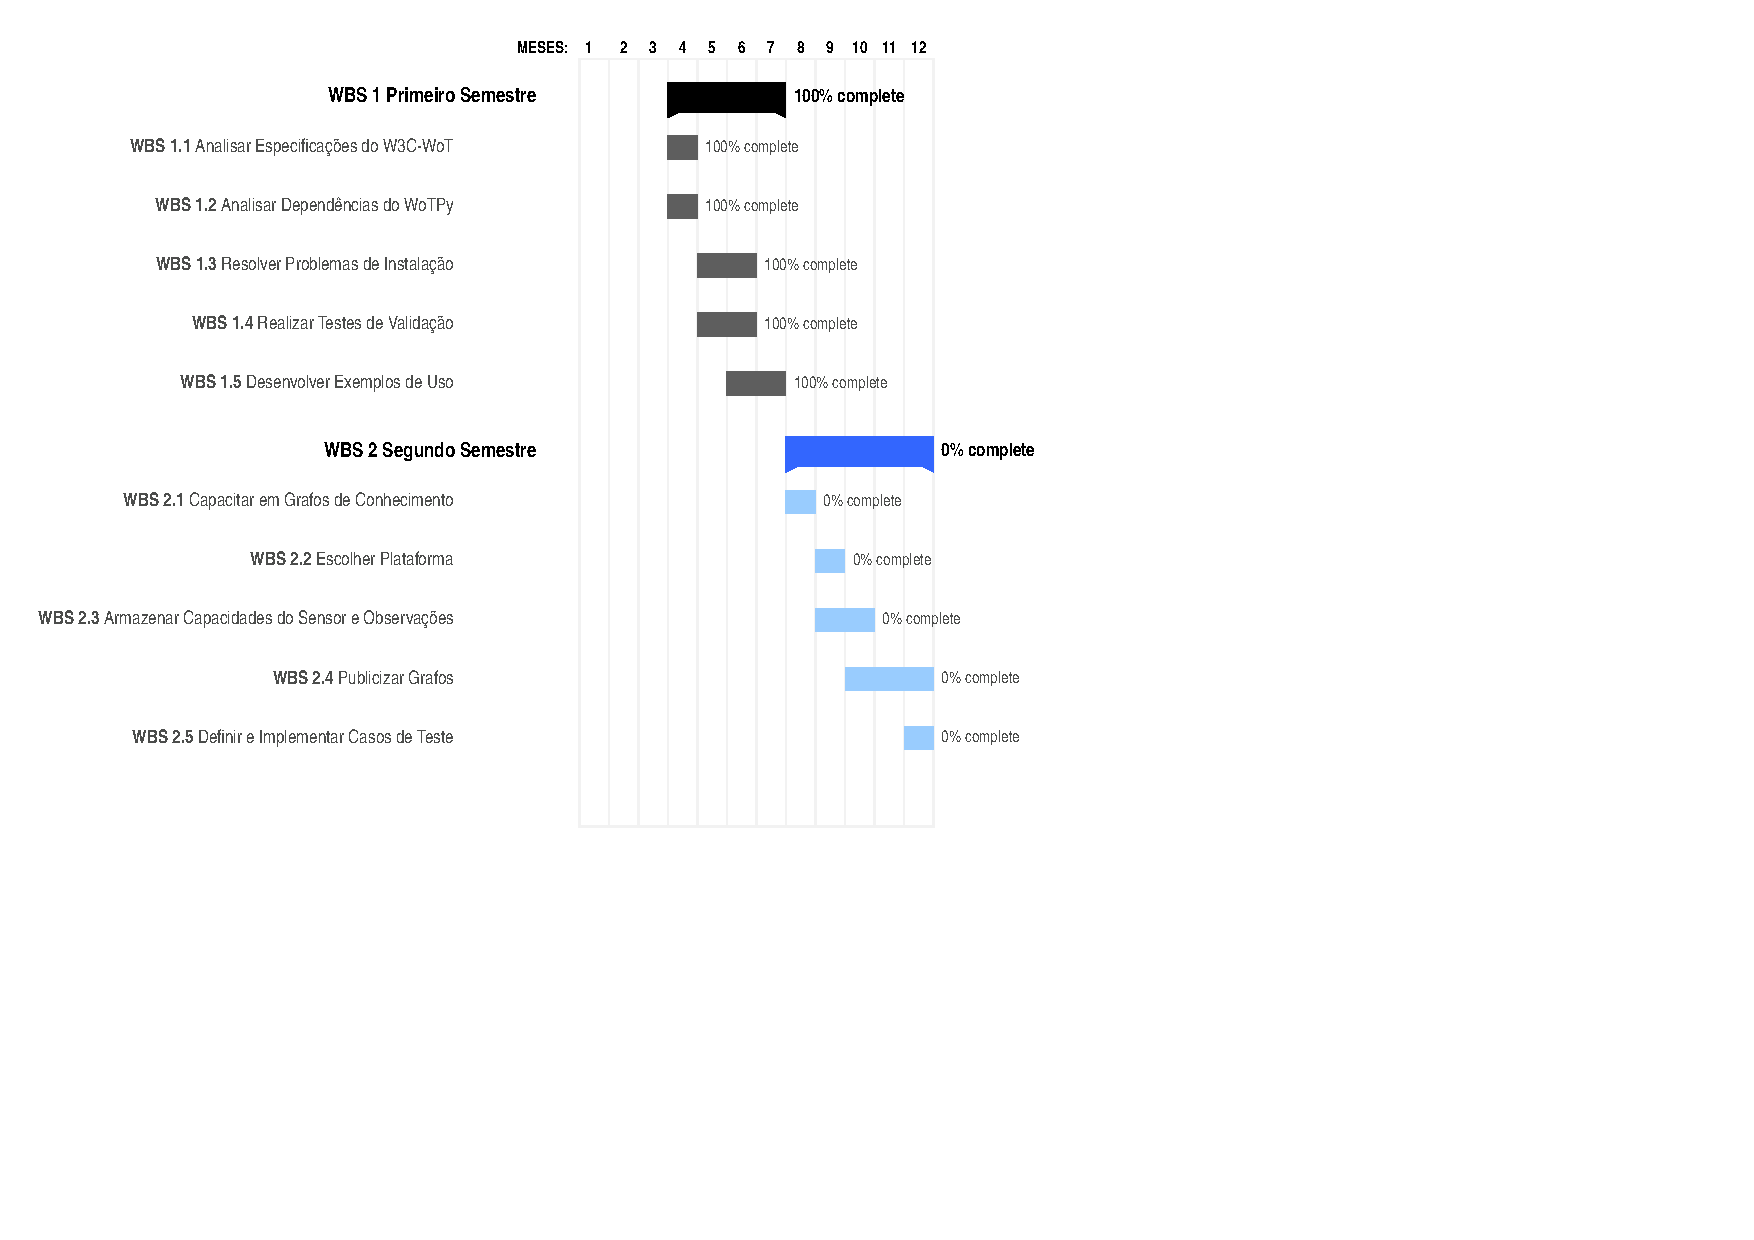
\includegraphics[trim={0.5cm 2.5cm 0 0 },clip]{figs/Cronograma_Ariga.pdf}
\end{figure}


% \chapter{Cronograma}

%
% https://www.overleaf.com/latex/examples/gantt-charts-with-the-pgfgantt-package/jmkwfxrnfxnw
% A fairly complicated example from section 2.9 of the package
% documentation. This reproduces an example from Wikipedia:
% http://en.wikipedia.org/wiki/Gantt_chart
%

\definecolor{barblue}{RGB}{153,204,254}
\definecolor{groupblue}{RGB}{51,102,254}
\definecolor{linkred}{RGB}{165,0,33}
\renewcommand\sfdefault{phv}
\renewcommand\mddefault{mc}
\renewcommand\bfdefault{bc}
\setganttlinklabel{s-s}{START-TO-START}
\setganttlinklabel{f-s}{FINISH-TO-START}
\setganttlinklabel{f-f}{FINISH-TO-FINISH}
\sffamily
\begin{adjustbox}{width=1.1\textwidth,center}
\begin{ganttchart}[
    canvas/.append style={fill=none, draw=black!5, line width=.75pt},
    hgrid style/.style={draw=black!5, line width=.75pt},
    vgrid={*1{draw=black!5, line width=.75pt}},
    today=4,
    today rule/.style={
      draw=black!64,
      dash pattern=on 3.5pt off 4.5pt,
      line width=1.5pt
    },
    today label font=\small\bfseries,
    title/.style={draw=none, fill=none},
    title label font=\bfseries\footnotesize,
    title label node/.append style={below=7pt},
    include title in canvas=false,
    bar label font=\mdseries\small\color{black!70},
    bar label node/.append style={left=2cm},
    bar/.append style={draw=none, fill=black!63},
    bar incomplete/.append style={fill=barblue},
    bar progress label font=\mdseries\footnotesize\color{black!70},
    group incomplete/.append style={fill=groupblue},
    group left shift=0,
    group right shift=0,
    group height=.5,
    group peaks tip position=0,
    group label node/.append style={left=.6cm},
    group progress label font=\bfseries\small,
    link/.style={-latex, line width=1.5pt, linkred},
    link label font=\scriptsize\bfseries,
    link label node/.append style={below left=-2pt and 0pt}
  ]{1}{12}
  \gantttitle[
    title label node/.append style={below left=7pt and -3pt}
  ]{MESES:\quad1}{1}
  \gantttitlelist{2,...,12}{1} \\
  
  \ganttgroup[progress=10]{WBS 1 Primeiro Semestre}{4}{7} \\
  \ganttbar[
    progress=30,
    name=WBS1A
  ]{\textbf{WBS 1.1} Analisar Especificações do W3C-WoT}{4}{4} \\
  \ganttbar[
    progress=40,
    name=WBS1B
  ]{\textbf{WBS 1.2} Analisar Dependências do WoTPy}{4}{4} \\
  \ganttbar[
    progress=0,
    name=WBS1C
  ]{\textbf{WBS 1.3} Resolver Problemas de Instalação}{5}{6} \\
  \ganttbar[
    progress=0,
    name=WBS1D
  ]{\textbf{WBS 1.4} Realizar Testes de Validação}{5}{6} \\
  \ganttbar[
    progress=0,
    name=WBS1E
  ]{\textbf{WBS 1.5} Desenvolver Exemplos de Uso}{6}{7} \\
  
  \ganttgroup[progress=0]{WBS 2 Segundo Semestre}{8}{12} \\
    \ganttbar[
    progress=0,
    name=WBS2A
  ]{\textbf{WBS 2.1} Capacitar em Grafos de Conhecimento}{8}{8} \\
  \ganttbar[
    progress=0,
    name=WBS2B
  ]{\textbf{WBS 2.2} Escolher Plataforma}{9}{9} \\
  \ganttbar[
    progress=0,
    name=WBS2C
  ]{\textbf{WBS 2.3} Armazenar Capacidades do Sensor e Observações}{9}{10} \\
  \ganttbar[
    progress=0,
    name=WBS2D
  ]{\textbf{WBS 2.4} Publicizar Grafos}{10}{12} \\
  \ganttbar[
    progress=0,
    name=WBS2E
  ]{\textbf{WBS 2.5} Definir e Implementar Casos de Teste}{12}{12} \\

  \ganttlink[link type=s-s]{WBS1A}{WBS1B}
  \ganttlink[link type=f-s]{WBS1B}{WBS1C}
  \ganttlink[link type=f-f]{WBS1C}{WBS1D}
  \ganttlink[link type=f-s]{WBS1D}{WBS1E}

  \ganttlink[link type=f-s]{WBS2A}{WBS2B}
  \ganttlink[link type=f-s]{WBS2B}{WBS2C}
  \ganttlink[link type=f-s]{WBS2C}{WBS2D}
  \ganttlink[link type=f-s]{WBS2D}{WBS2E}
  
  % \ganttlink[
    % link type=f-f,
    % link label node/.append style=left
  % {WBS1C}{WBS1D}
  
\end{ganttchart}
\end{adjustbox}

%
% A simpler example from the package documentation:
%

% \begin{ganttchart}{1}{12}
  % \gantttitle{2011}{12} \\
  % \gantttitlelist{1,...,12}{1} \\
  % \ganttgroup{Group 1}{1}{7} \\
  % \ganttbar{Task 1}{1}{2} \\
  % \ganttlinkedbar{Task 2}{3}{7} \ganttnewline
  % \ganttmilestone{Milestone}{7} \ganttnewline
  % \ganttbar{Final Task}{8}{12}
  % \ganttlink{elem2}{elem3}
  % \ganttlink{elem3}{elem4}
% \end{ganttchart}

% \end{document}

No início do primeiro semestre, uma análise detalhada das especificações do W3C-WoT será realizada (\ref{estudo}), seguida pela seleção e estudo das bibliotecas e ferramentas relevantes para o projeto (\ref{dependência}) Em paralelo, serão identificados e resolvidos problemas de instalação do WoTPy (\ref{instalação}). Com as melhorias implementadas, serão realizados testes e validações para garantir a qualidade e a funcionalidade das contribuições feitas (\ref{teste}).

No final do primeiro semestre, serão desenvolvidos exemplos de uso e documentação detalhada do projeto (\ref{uso}), auxiliando desenvolvedores e usuários na implementação do WoTPy em seus próprios projetos IoT. O exemplo prático incluirá ajustes na comunicação do dispositivo Protetor Solar (ou similar).

Para o segundo semestre, o que se espera inclui a capacitação em ferramentas de grafos de conhecimento, a escolha de uma plataforma de armazenamento para esses grafos, o armazenamento das capacidades do sensor em SSN e das observações em SOSA, a publicização desses grafos por meio de um endpoint SPARQL e a definição e implementação de casos de teste para a integração.



%
% https://www.overleaf.com/latex/examples/gantt-charts-with-the-pgfgantt-package/jmkwfxrnfxnw
% A fairly complicated example from section 2.9 of the package
% documentation. This reproduces an example from Wikipedia:
% http://en.wikipedia.org/wiki/Gantt_chart
%


% \definecolor{barblue}{RGB}{153,204,254}
% \definecolor{groupblue}{RGB}{51,102,254}
% \definecolor{linkred}{RGB}{165,0,33}
% \renewcommand\sfdefault{phv}
% \renewcommand\mddefault{mc}
% \renewcommand\bfdefault{bc}
% \setganttlinklabel{s-s}{START-TO-START}
% \setganttlinklabel{f-s}{FINISH-TO-START}
% \setganttlinklabel{f-f}{FINISH-TO-FINISH}
% \sffamily
% \begin{figure}
%     \caption{Cronograma}
%     \label{fig:cronograma}
% \begin{adjustbox}{width=1.1\textwidth,center}
% \begin{ganttchart}[
%     canvas/.append style={fill=none, draw=black!5, line width=.75pt},
%     hgrid style/.style={draw=black!5, line width=.75pt},
%     vgrid={*1{draw=black!5, line width=.75pt}},
%     today=4,
%     today rule/.style={
%       draw=black!64,
%       dash pattern=on 3.5pt off 4.5pt,
%       line width=1.5pt
%     },
%     today label font=\small\bfseries,
%     title/.style={draw=none, fill=none},
%     title label font=\bfseries\footnotesize,
%     title label node/.append style={below=7pt},
%     include title in canvas=false,
%     bar label font=\mdseries\small\color{black!70},
%     bar label node/.append style={left=2cm},
%     bar/.append style={draw=none, fill=black!63},
%     bar incomplete/.append style={fill=barblue},
%     bar progress label font=\mdseries\footnotesize\color{black!70},
%     group incomplete/.append style={fill=groupblue},
%     group left shift=0,
%     group right shift=0,
%     group height=.5,
%     group peaks tip position=0,
%     group label node/.append style={left=.6cm},
%     group progress label font=\bfseries\small,
%     link/.style={-latex, line width=1.5pt, linkred},
%     link label font=\scriptsize\bfseries,
%     link label node/.append style={below left=-2pt and 0pt}
%   ]{1}{12}
%   \gantttitle[
%     title label node/.append style={below left=7pt and -3pt}
%   ]{MESES:\quad1}{1}
%   \gantttitlelist{2,...,12}{1} \\
  
%   \ganttgroup[progress=100]{WBS 1 Primeiro Semestre}{4}{7} \\
%   \ganttbar[
%     progress=100,
%     name=WBS1A
%   ]{\textbf{WBS 1.1} Analisar Especificações do W3C-WoT}{4}{4} \\
%   \ganttbar[
%     progress=100,
%     name=WBS1B
%   ]{\textbf{WBS 1.2} Analisar Dependências do WoTPy}{4}{4} \\
%   \ganttbar[
%     progress=100,
%     name=WBS1C
%   ]{\textbf{WBS 1.3} Resolver Problemas de Instalação}{5}{6} \\
%   \ganttbar[
%     progress=100,
%     name=WBS1D
%   ]{\textbf{WBS 1.4} Realizar Testes de Validação}{5}{6} \\
%   \ganttbar[
%     progress=100,
%     name=WBS1E
%   ]{\textbf{WBS 1.5} Desenvolver Exemplos de Uso}{6}{7} \\
  
%   \ganttgroup[progress=0]{WBS 2 Segundo Semestre}{8}{12} \\
%     \ganttbar[
%     progress=0,
%     name=WBS2A
%   ]{\textbf{WBS 2.1} Capacitar em Grafos de Conhecimento}{8}{8} \\
%   \ganttbar[
%     progress=0,
%     name=WBS2B
%   ]{\textbf{WBS 2.2} Escolher Plataforma}{9}{9} \\
%   \ganttbar[
%     progress=0,
%     name=WBS2C
%   ]{\textbf{WBS 2.3} Armazenar Capacidades do Sensor e Observações}{9}{10} \\
%   \ganttbar[
%     progress=0,
%     name=WBS2D
%   ]{\textbf{WBS 2.4} Publicizar Grafos}{10}{12} \\
%   \ganttbar[
%     progress=0,
%     name=WBS2E
%   ]{\textbf{WBS 2.5} Definir e Implementar Casos de Teste}{12}{12} \\

%   \ganttlink[link type=s-s]{WBS1A}{WBS1B}
%   \ganttlink[link type=f-s]{WBS1B}{WBS1C}
%   \ganttlink[link type=f-f]{WBS1C}{WBS1D}
%   \ganttlink[link type=f-s]{WBS1D}{WBS1E}

%   \ganttlink[link type=f-s]{WBS2A}{WBS2B}
%   \ganttlink[link type=f-s]{WBS2B}{WBS2C}
%   \ganttlink[link type=f-s]{WBS2C}{WBS2D}
%   \ganttlink[link type=f-s]{WBS2D}{WBS2E}
  
  % \ganttlink[
    % link type=f-f,
    % link label node/.append style=left
  % {WBS1C}{WBS1D}
  
% \end{ganttchart}
% \end{adjustbox}
% \end{figure}

